% \documentclass{minimal}
% \usepackage{pgfplots}
% \begin{document}

\pgfplotsset{width=\textwidth}
\centering
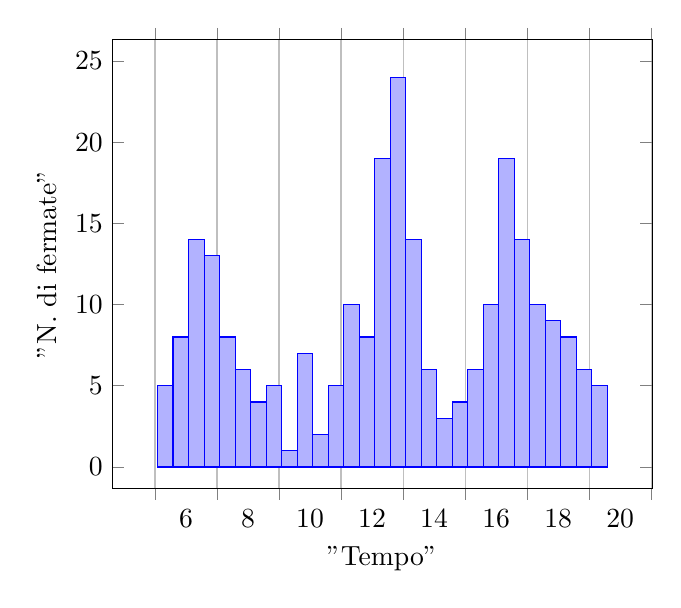
\begin{tikzpicture}
\begin{axis}[xlabel="Tempo", ylabel="N. di fermate",%
ybar interval,
xtick=,% reset from ybar interval%
% ybar,bar width=6pt
]
\addplot
coordinates
{
(6.0833, 5) (6.5833, 8) (7.0833, 14) (7.5833, 13) (8.0833, 8) (8.5833, 6) (9.0833, 4) (9.5833, 5) (10.0833, 1) (10.5833, 7) (11.0833, 2) (11.5833, 5) (12.0833, 10) (12.5833, 8) (13.0833, 19) (13.5833, 24) (14.0833, 14) (14.5833, 6) (15.0833, 3) (15.5833, 4) (16.0833, 6) (16.5833, 10) (17.0833, 19) (17.5833, 14) (18.0833, 10) (18.5833, 9) (19.0833, 8) (19.5833, 6) (20.0833, 5) (20.5833, 2)
};
\end{axis}
\end{tikzpicture}

% \end{document}